
        \DocumentMetadata{
        pdfversion=1.7,
        pdfstandard=A-3b,
        }
        \documentclass[a4paper]{article}
        %To support embedding of a file in the PDF/A-3
        \usepackage{embedfile}
        \embedfilesetup{     
            filesystem=URL, 
            mimetype=application/octet-stream, % Defined syntax to embed excel files
            afrelationship={/Data}, %Relationship of the pdf to the embedded file is data
            stringmethod = escape %Treats an unknown symbol as an escape character
        }

        %%%%%% Packages included %%%%%%
        
        %% Language and font encoding
        \usepackage[english]{babel}
        \usepackage{textcomp} %For special symbols
        % To support Hindi symbols
        \usepackage[T1]{fontenc} 
        \usepackage{fontspec}
        \usepackage{polyglossia}
        \setmainlanguage{english} % Continue using english for rest of the document
        \setotherlanguages{hindi} % To use \texthindi to write Hindi in the document
        \newfontfamily\hindifont{Noto Sans Devanagari}[Script=Devanagari] %For Hindi script
        \setmainfont{Arial}% Set Arial as the default font
        \usepackage{longtable} % To split table if it doesn't fit in one page
        \usepackage[scaled]{uarial} % Load the uarial package to use Arial font
        \usepackage[a4paper]{geometry} %To define dimensions of the page
        \usepackage{emptypage}	%To remove header and footer from the last page
        \usepackage{siunitx} %SI units representation
        \usepackage{array}  % for specifying column alignment
        \usepackage{makecell}  % for formatting cells
        \usepackage{xcolor} %To define the color of text
        \usepackage{multirow}%For more flexibility in tables
        \usepackage{multicol}%For more flexibility in tables
        \usepackage{background} %To create a watermark
        \usepackage{tcolorbox} %To use parbox and wrap text
        \usepackage{graphicx} %To include images
        \usepackage{tabularx} %For tables
        \usepackage{lastpage} % For number of pages
        \usepackage{fancyhdr}%header & footer
        \usepackage{setspace} % For setting line spacing
        \usepackage{float} % Aligns the tables to the top for better space utilization

        


        %%%%% Page format %%%%%%%
        
        % Adjust margins
        \geometry{
            top=0.9cm,
            bottom=10.7cm,
            left=0.7cm,
            right=0.7cm
        }

        \pagestyle{fancy} %Defining the page style 
        \fancyhf{}  %Clear the header and footer
        \newcounter{rownum} % Create a new counter to count the number of headings given
        \renewcommand{\headrulewidth}{0pt}	%No line below the header
        \renewcommand\footrule{\hrule width 19.65cm height 0.5mm} %To have a line above footer with the specified dimensions

        \newcommand{\fullhline}{\noalign{\hrule height 0.8mm}} %To have a thick horizontal line for selective columns

        % Set column separation
        \setlength{\tabcolsep}{0pt} %To remove the inter-column space


        % Define watermark
        \backgroundsetup{
        scale=1.02,  % Scale the watermark
        opacity=0.05,  % Opacity of the watermark (1 = opaque, 0 = fully transparent)
        angle=0,  % Angle of the watermark
        position=current page.center,  % Position of the watermark
        vshift=-0.6cm,  % Vertical shift of the watermark
        hshift=-0.2mm,  % Horizontal shift of the watermark
        contents={%
            
\includegraphics[width=10cm,height=10cm]{./static/pdf_images/Logo_NPL_india.png}  % Path to your watermark image
        }
        }
        


        %%% HEADER %%%
        
            \fancyhead[L]{
            \begin{minipage}{13.4cm}
            \begin{spacing}{0.6}
            \begin{tabular}{>{\centering}m{2.2cm} >{\centering}m{9 cm} >{\centering\arraybackslash} m{2.1 cm}}

            
\includegraphics[width=3cm, height=3cm]{./static/pdf_images/CSIR_logo.png}		&	\makecell[bc]{\fontsize{11}{12}\selectfont \textbf{\texthindi{सी एस आई आर- राष्ट्रीय भौतिक प्रयोगशाला}}\\\fontsize{11}{12}\selectfont \textbf{CSIR-NATIONAL PHYSICAL LABORATORY}\\\fontsize{8}{12}\selectfont \texthindi{(वैज्ञानिक और औद्योगिक अनुसंधान परिषद)}\\\fontsize{9}{12}\selectfont (Council of Scientific and Industrial Research)\\\fontsize{6}{12}\selectfont \texthindi{(राष्ट्रीय मापिकी विज्ञान संस्थान (एनएमआई), सदस्य बीआईपीएम एवं हस्ताक्षरकर्ता सीआईपीएम --एमआरए)}\\\fontsize{6}{12}\selectfont \textbf{(National Metrology Institute (NMI), Member BIPM and Signatory CIPM - MRA)}\\\fontsize{6}{12}\selectfont \textbf{\texthindi{डॉ के एस कृष्णन मार्ग, नई दिल्ली-110012, भारत}}\\\fontsize{6}{12}\selectfont \textbf{Dr. K. S. Krishnan Marg, New Delhi-110012, INDIA}\\\fontsize{6}{12}\selectfont \texthindi{दूरभाष}\textbf{/Phone : 91-11-4560 8441, 8589, 8610, 9447,}\texthindi{फैक्स}\textbf{/Fax : 91-11-4560 8448}\\\fontsize{6}{12}\selectfont \texthindi{ई-मेल}\textbf{/E-mail: cfct@nplindia.org,} \texthindi{वेबसाईट}\textbf{/Website: www.nplindia.org}}	&	\hspace{-0.6cm}\raisebox{0.6cm}{
\includegraphics[width=2.35cm, height=2.35cm]{./static/pdf_images/Logo_NPL_india.png}}\\
            \end{tabular}
            \end{spacing}
            \end{minipage}%
            \begin{minipage}{6.2cm}
            \centering
            \setlength{\arrayrulewidth}{0.8mm}
            \begin{tabular}{|>{\centering\arraybackslash}p{6.2 cm}}
            \makecell{\texthindi{परीक्षण रिपोर्ट}\\\textbf{TEST REPORT}}\\
            \begin{minipage}{6.2cm}\centering{Raman Analysis of given sample}\end{minipage}\\[0.5cm]
            \hline
            \makecell{\texthindi{डी ओ आई संख्या}/DOI number :\vspace{0.15cm}\\ X }\\[0.5cm]

            \end{tabular}
            \end{minipage}
            \begin{tabular}{>{\centering}p{3.8cm}!{\vrule width 0.8mm}>{\centering}p{8.3cm}!{\vrule width 0.8mm}>{\centering}p{2.5cm}!{\vrule width 0.8mm}>{\centering\arraybackslash}p{4.9cm}}
            \fullhline
            \texthindi{दिनंक}/\textbf{Date} & \texthindi{परीक्षण रिपोर्ट संख्या}/\textbf{Test Report No.} & \texthindi{पृष्ठ}/\textbf{Page} & \texthindi{पृष्ठों की संख्या}/\textbf{No of pages}\\
            23.12.2019&N19110969/D1.06/T-272&\thepage&\pageref{LastPage}\\[1.8ex]
            \fullhline
            \end{tabular}
            }
            

        %%% FOOTER %%%
        
            \fancyfoot[C]{
            \begin{minipage}{\textwidth}
            \centering
            \begin{tabular}{ p{3.5 cm} p{3.5 cm} p{3.5 cm} p{3.5 cm} p{3.5 cm} p{3.5 cm} }
            \makecell[lb]{\texthindi{परीक्षाणकर्ता}\\\textbf{Tested by :} } & \parbox[t][0.5cm][l]{2cm}{
\includegraphics[width=1.8cm, height=0.8cm]{./signatures/calibrated_by.jpg}}
            & \makecell[lb]{\texthindi{जाँचकर्ता}\\\textbf{Checked by :} } & \parbox[t][0.5cm][l]{2cm}{
\includegraphics[width=1.8cm, height=0.8cm]{./signatures/checked_by.jpg}}
            & \makecell[lb]{\texthindi{प्रभारी वैज्ञानिक}\\ \textbf{Scientist-in-charge :} } & \parbox[t][0.5cm][l]{2cm}{
\includegraphics[width=1.8cm, height=0.8cm]{./signatures/incharge.jpg}}\\
            \multicolumn{2}{c}{(JASVEER SINGH)} & \multicolumn{2}{c}{(Dr. NITA DILAWAR SHARMA)} & \multicolumn{2}{c}{Dr. Sushil Kumar} \\[1.5 ex]
            \\
            & & \makecell[lb]{\texthindi{जारिकर्ता}\\\textbf{Issued by :}} & \parbox[t][0.5cm][l]{2cm}{
\includegraphics[width=1.8cm, height=0.8cm]{./signatures/issued_by.jpg}} & &\\
            & & \multicolumn{2}{c}{(Dr. SANJAY YADAV)} & & \\
            \end{tabular}
            \end{minipage}
            }
            

        \setlength{\headheight}{6.9cm}
        \setlength{\footskip}{1.95cm}


        %%%%%% DOCUMENT BEGINS HERE  %%%%%%%%%%
        \begin{document}
        
        %%%% Administrative Data %%%%%%%
        
            \headsep = 0cm
            \small
            
            {
            \renewcommand{\arraystretch}{2.4}
            \hspace{0.95cm}
            \begin{tabular}{p{1cm} p{6.74cm}  p{0.5cm} p{8cm}}
            \stepcounter{rownum}\arabic{rownum}. 	&	\makecell[l]{Tested for}		&:&	\parbox[t]{7.8cm}{\raggedright Biomedical Instrumentation Metrology Section  \\
CSIR-National Physical Laboratory.  \\
Dr. K.S. Krishnan Marg, New Delhi-110012  \\
Customer's Ref. No.: CTR Form, Dated: 25.11.19} \\
            \stepcounter{rownum}\arabic{rownum}. 	&	\makecell[lt]{Description and Identification \\of Sample}  &:&	\parbox[t]{7.8cm}{ \raggedright Graphene Oxide, Identification no. Gl} \\
            \stepcounter{rownum}\arabic{rownum}.	&	\makecell[lt]{Environmental Conditions} 	& :&	 \begin{minipage}[t]{7.8cm}{\raggedright Temperature: (23 \textpm 2) °C  \\
Relative Humidity: (50 \textpm 10)\%} \end{minipage}\\
            \stepcounter{rownum}\arabic{rownum}.	&	\makecell[lt]{Standard(s) used (with)\\ Associated Uncertainty}  &:& \begin{minipage}[t]{7.8cm}{\raggedright The spectrometer was calibrated for wavelength using standard silicon and diamond samples.} \end{minipage}\\
            \stepcounter{rownum}\arabic{rownum}.	&	\makecell[lt]{Traceability of Standard(s) used}	&:&	\parbox[t]{7.8cm}{ \raggedright } \\
            \stepcounter{rownum}\arabic{rownum}.	&	\makecell[lt]{Principle /Methodology of Test and\\Test Procedure number} 	& :&	\parbox[t]{7.8cm}{\raggedright The sample is irradiated by argon ion laser of 514.5 nm wavelength and the scattered radiation collected in the back-scattering geometry was analyzed using a triple monochromator coupled with charge coupled device (CCD).} \\
            \end{tabular}
            }
            

        \newpage

        %%%%%% Measurement Data %%%%%%%%
        
            \hspace{0.95cm}
            \begin{tabular}{p{1cm} p{6.74cm}}
            \stepcounter{rownum}\arabic{rownum}. & Result(s): \\
            \end{tabular}
            {
            \renewcommand{\arraystretch}{1.3}
            
            }

            %%%%%%%%%%%%%% Conditional graph plotting %%%%%%%%%%%%%%%%
            
        \vspace{0.2 cm}
        \hspace{0.8 cm}\textbf{Sample:} Graphene Oxide, Identification no. Gl\\
        \begin{center}
        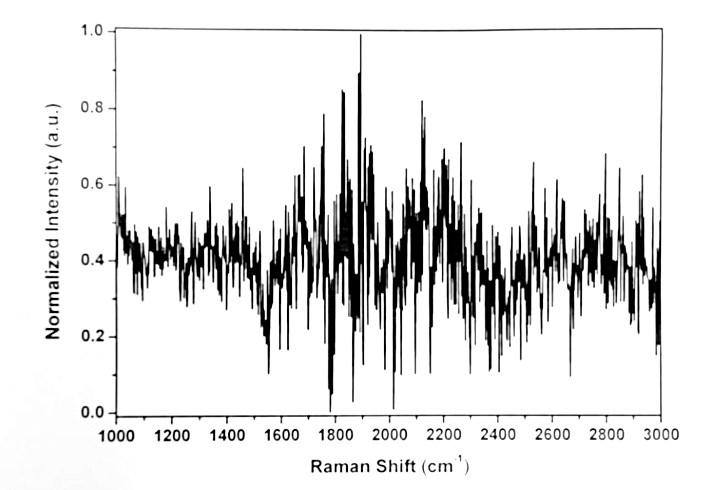
\includegraphics[width=0.6\textwidth]{./static/pdf_images/graph.png}\\
        \end{center}
        

            \hspace{0.8 cm}\begin{minipage}[c]{0.85\textwidth}
            The Raman spectrum of the sample shows the normalized intensity with Raman shift. The peaks represent the various vibrational modes of the given sample.
            \end{minipage}\\
            %%%%%%%%% Date and Remarks %%%%%%%%%%
            {
            \renewcommand{\arraystretch}{2.4}
            \hspace{0.95cm}
            \begin{tabular}{p{1cm} p{6.74cm} p{8cm}}
            \stepcounter{rownum}\arabic{rownum}. 	&	Date(s) for Testing: &	23.12.2019 \\
            \stepcounter{rownum}\arabic{rownum}.		&	Remark(s):	&	\parbox[t]{8.5cm}{\raggedright The data file is also being provided separately in electronic form.}   \\
            \end{tabular}
            }
            


        %%%%%%% LAST PAGE %%%%%%%%%%%
        
        \AtEndDocument{ %To keep this at the end of the document
        \newpage %Gives a fresh page
        \thispagestyle{empty} %Clears all the headers
        \newgeometry{top=2cm, bottom=2.4cm, left=1.2cm, right=1.2cm }  % Redefine the margins
        \backgroundsetup{contents={}} % Removes the watermark
        \renewcommand{\seriesdefault}{\bfdefault} % Change the default font style to bold
        \setmainfont{Arial} % Change the default font family to Arial
        \Large %Textsize: 14.4

        \begin{center}\LARGE \texthindi{नोट}\end{center} %Heading of size: 17.28 in the center of the page
        \begin{spacing}{0.8}
        \begin{enumerate}
        \item \texthindi{यह प्रमाण पत्र सी एस आई आर-राष्ट्रीय भौतिक प्रयोगशाला, भारत जारी किया गया है जौ कि विज्ञान एवं प्रौद्योगिकी मंत्रालय, भारत सरकार के अधीन वैज्ञानिक व औद्योगिक अनुसंधान परिषद्‌ की संघटक इकाई है एवम्‌ भारत का राष्ट्रीय मापिकी  संस्थान}(NMI) \texthindi{ भी है ।}
        \item \texthindi{यह प्रमाण पत्र केवल अंशांकन हेतु जमा किएं गए माषिकी हेतु संदर्थित है।}
        \item \texthindi{इस प्रमाण पत्र की प्रतिलिपी, पूर्ण प्रमाण पत्र के अतिरिक्त, तैयार नहीं की जा सकती है, जब तक कि निदेशक, सी एस आई आर-राष्ट्रीय भौतिक प्रयोगशाला, नई दिल्‍ली से अनुमोदित सार के प्रकाशन हेतु लिखित अनुमति प्राप्त नहीं की गयी हो।}
        \item \texthindi{उस प्रमाण पत्र में प्रतिवेदित परीक्षण परिणाम केवल मापन की वर्णित परिस्थलियाँ एवं समय हेतु मान्य है।}
        \end{enumerate}
        \end{spacing}

        \vfill    %Ensures that elements are evenly spaced and spread out
        \centering 
\includegraphics[width=10cm, height=10cm]{./static/pdf_images/NPL_logo_gray.jpeg} %Includes photo
        \vfill %Ensures that elements are evenly spaced and spread out

        \begin{center}\LARGE NOTE\end{center} %Heading of size: 17.28 in the center of the page
        \begin{spacing}{0.8}
        \begin{enumerate}
        \item This certificate is issued by CSIR-National Physical Laboratory of India (NPLI) which is a constituent unit of the Council of Scientific \& Industrial Research, the Ministry of Science and Technology, Government of India and is also National Metrology Institute (NMI) of India.
        \item This certificate refers only to the particular item (s) submitted for calibration.
        \item This certificate shall not be reproduced, except in full, unless written permission for the publication of an approved abstract has been obtained from the Director, CSIR- National Physical Laboratory. New Delhi.
        \item The calibration results reported in this certificate are valid at the time and under the stated conditions of measurement.
        \end{enumerate}
        \end{spacing}
        }
        

        \embedfile{./excel_files/N19110969_D1.06_T-272.xlsx}
        \end{document}
        